% !TEX encoding = UTF-8 Unicode
\RequirePackage{fix-cm}
\documentclass[a4paper,10pt,UTF8]{paper}
%\documentclass[a4paper,10pt,UTF8]{ctexart}

\usepackage[english]{babel}
\usepackage{fancyhdr,array,lastpage,amsmath,mathtools,enumitem,graphicx,multirow,tocbibind,longtable,makecell,varwidth,titlesec,bm,booktabs,comment}
\usepackage{enumitem}
\usepackage{hyperref}
\hypersetup{hidelinks}
%\setCJKmainfont[BoldFont=Heiti SC Medium]{Songti SC Light}
%\setCJKsansfont{Heiti SC}

\usepackage[left=2.54cm,right=2.54cm,top=2.54cm,bottom=2.54cm]{geometry}
\usepackage[font=footnotesize,labelfont=bf]{caption}
\usepackage{tikz,flowchart}
\usepackage{ctex}
\usetikzlibrary{shapes,shapes.geometric,arrows,matrix,calc}
\usetikzlibrary{circuits.logic}
% \usetikzlibrary{circuits.logic.custom}
\usetikzlibrary{circuits.logic.IEC}
\usetikzlibrary{shadows}
\usepackage{listings}
\usepackage[Q=yes]{examplep}
\usepackage{fancyhdr}
\usepackage{alphalph}
\usepackage{indentfirst}

\newenvironment{sol}
  {\par\vspace{2mm}\noindent{\bf Solution}. }

\lstset{escapeinside=``, breaklines=true, frame=none, extendedchars=false, basicstyle=\ttfamily, showstringspaces=false}


\setlength{\parindent}{2em}
\setlength{\parskip}{1.5ex plus 0.5ex minus 0.2ex}
\linespread{1.1}

\bibliographystyle{plain}

\numberwithin{equation}{section}
\numberwithin{figure}{section}

\usepackage{karnaugh}
\usepackage{circuitikz}


\setcounter{secnumdepth}{3}
\setcounter{tocdepth}{3}

\title{华东师范大学计算机科学技术系上机实验报告}

\begin{document}
\pagestyle{fancy}
\chead{\small\color{gray}华东师范大学计算机科学技术系上机实验报告}
\lhead{}
\rhead{}
\makeatletter
\def\headrule{{\if@fancyplain\let\headrulewidth\plainheadrulewidth\fi%
\color{gray}\hrule\@height 0.2pt\@width\headwidth}
  \vspace{6mm}}
\makeatother

\newcommand{\HRule}{\rule{\linewidth}{1mm}}
\newcommand{\dai}{\textbf{Dais-CMX16$^+$}}

{\center {\huge \bfseries \LARGE{华东师范大学计算机科学技术系上机实验报告}} \\ [0.8cm]

\small{
  \begin{minipage}[t]{.32\linewidth}
    \textbf{课程名称:}计算机组成与结构实践\\
    \textbf{指导教师:}金健\\
    \textbf{上机实践名称:}准双向I/O口和通用寄存器实验\\
    \textbf{实践编号:}实验 1
  \end{minipage}
  \begin{minipage}[t]{.32\linewidth}
    \textbf{年级:}17 级\\
    \textbf{姓名:}朱桐\\
    \textbf{学号:}10175102111\\
    \textbf{组号:}A
  \end{minipage} 
  \begin{minipage}[t]{.32\linewidth}
    \textbf{上机实践成绩:} \\
    \textbf{创新实践成绩:} \\
    \textbf{上机实践日期:}2019/09/20\\
    \textbf{上机实践时间:}2 学时\\
  \end{minipage}
}
\HRule \\[0.5cm]
}
\section{实验目的}

\begin{enumerate}
    \item 了解两种控制方式:“手动”和“微控制”
    \item 了解两种实验方式:“搭接”和“在线”
    \item 理解并学会设置手动搭接实验方式
    \item 熟悉与了解准双向 I/O 口的构成原理
    \item 掌握准双向 I/O 口的输入/输出特性的运用
    \item 熟悉通用寄存器的数据通路
    \item 掌握通用寄存器的构成和运用
\end{enumerate}

\section{实验设备}

\dai 设备,导线若干

\section{实验内容}

在手动控制模式和搭接实验方式下,实现 I/O 经由总线到寄存器以及寄存器经由总线到 I/O 的数据传输,以及在不同模式(奇数位和偶数位)之间的转换。

\section{实验原理}

\subsection{总线}

总线(Bus)是计算机各种功能部件之间传送信息的公共通信干线,它是由导线组成的传输线束, 按照计算机所传输的信息种类,计算机的总线可以划分为数据总线、地址总线和控制总线,分别用来传输数据、数据地址和控制信号。总线是一种内部结构,它是cpu、内存、输入、输出设备传递信息的公用通道,主机的各个部件通过总线相连接,外部设备通过相应的接口电路再与总线相连接,从而形成了计算机硬件系统。在计算机系统中,各个部件之间传送信息的公共通路叫总线,微型计算机是以总线结构来连接各个功能部件的。

从I/O到寄存器以及从寄存器到I/O的数据都要经过总线。各种部件与总线连接,不同部件完成不同功能,数据通过总线从一个部件到达另一个部件。

\subsection{源部件与目的部件}

源部件和目的部件一般只有一路数据到达,否则,部件将难以判断应该处理哪一路数据。比如一个 MIPS 指令

\subsection{字与字节}

在16位计算机中,一个字 (word) 等于两个字节 (byte)

在\dai 计算机中,我们可以一次传输一个字,也可以把16位的高8位当作奇字节,低8位当作偶字节。

\subsection{开关信号:常开与脉冲}

在通常情况下,由部件到总线是由常开开关决定的,因此部件的输入一般会实时更新总线上的数据。在实际实验时,改变 I/O 口,总线上的数据也会及时更新。总线到部件上则是由脉冲控制,脉冲发生时,数据输出到部件。

\subsection{寄存器组}

本次实验用到的是两个通用寄存器组CX和DX。

\subsection{数据通路}

\dai 向用户提供的是按准双向原理设计的十六位输入/输出 I/O 口,当该位为“1”
时才能用作输入源,上电或复位(手动态按【返回】键),该十六位 I/O 口被置位(即为“FFFFh”)。
通常情况下,在用作输入的时候就不能再有输出定义。电路结构如图 \ref{fig:io} 所示。该口外接十六
位二进制数据开关,适用于外部数据的输入,该口跨接十六个发光二极管,经缓冲驱动四个七段
显示,能以二进制和十六进制两种方式显示 I/O 口的输入输出状态。发光管在高电平“1”时发
光点亮。

\begin{figure}[h]
    \centering
    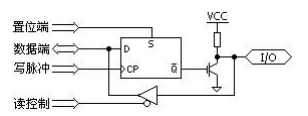
\includegraphics[width=0.7\textwidth]{io.PNG}
    \caption{准双向I/O电路}
    \label{fig:io}
\end{figure}{}

实验中所用的 I/O 口数据通路如图 \ref{fig:circuit} 所示。I/O 的输入经 2 片 74LS245 缓冲与数据总线
相连,I/O 口的输出由 2 片 74LS574 锁存后输出,锁存器的输入端与数据总线相连。

\begin{figure}[h]
    \centering
    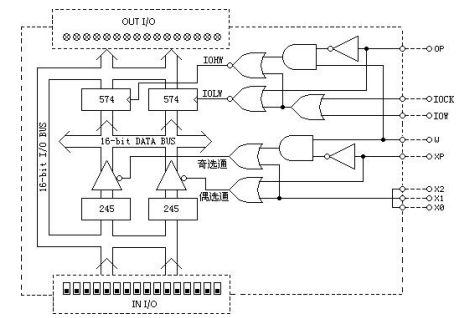
\includegraphics[width=0.7\textwidth]{circuit.PNG}
    \caption{I/O口数据通路}
    \label{fig:circuit}
\end{figure}{}


\section{实验步骤}

\subsection{初始化}

\subsubsection{工作模式设置}

在初始待令状态下,按【减址】键,LCD 显示器提示工作模式选项:
按【增址】键,将光标移到“KLD”单元手动模式,按【减址】键确定后,询问用户是否使
用搭接方式的选项。操作过程如图 \ref{fig:dajie} 所示。

\subsubsection{初始化操作}

一旦进入手控状态,首先应把实验系统左下方“二进制开关单元”的24 位微控制开关拨至
下方(即低电平信号“0”),使24 位微控制状态指示灯熄灭,关闭全部控制信号,完成微控制器
的初始化操作。

\begin{figure}[h]
    \centering
    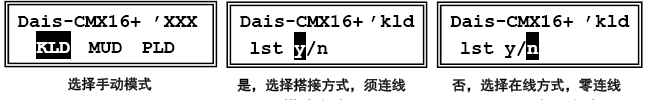
\includegraphics[width=1\textwidth]{dajiemoshi.PNG}
    \caption{搭接模式}
    \label{fig:dajie}
\end{figure}

\subsection{控制信号}

$X_2X_1X_0$ 是总线的输入控制信号,用导线将其接到信号开关上以便手动控制。

$W, XP, OP$ 分别是传输位长(是否输出高8位),输入奇偶位控制和输出部件奇偶位控制。奇偶位控制置为1时,输出偶位。
不过如果位长控制位和奇偶位控制位同时为0,则输入输出高8位。

$RXW, IOW$ 分别控制寄存器读入和 I/O 口输出。当 $RXW=1$,总线输入通用寄存器,否则设置好合适的 $X_2X_1X_0$ 寄存器会输入到总线。$IOW$ 同理,置为1时I/O输出,此时应该把所有开关置为1。
\subsubsection{搭接方式}

\begin{figure}[h]
    \centering
    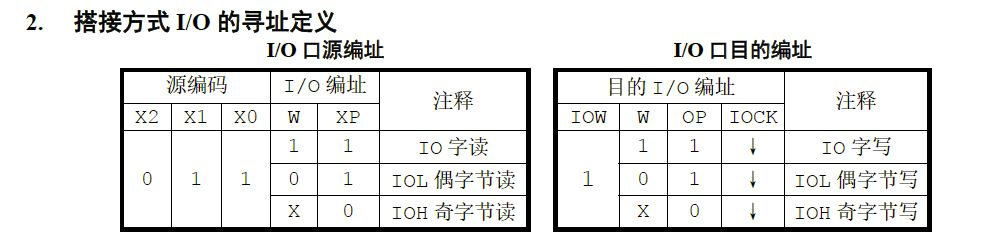
\includegraphics[width=1\textwidth]{dajie.JPG}
    \caption{寻址定义}
    \label{fig:xunzhi}
\end{figure}

\begin{figure}[h]
    \centering
    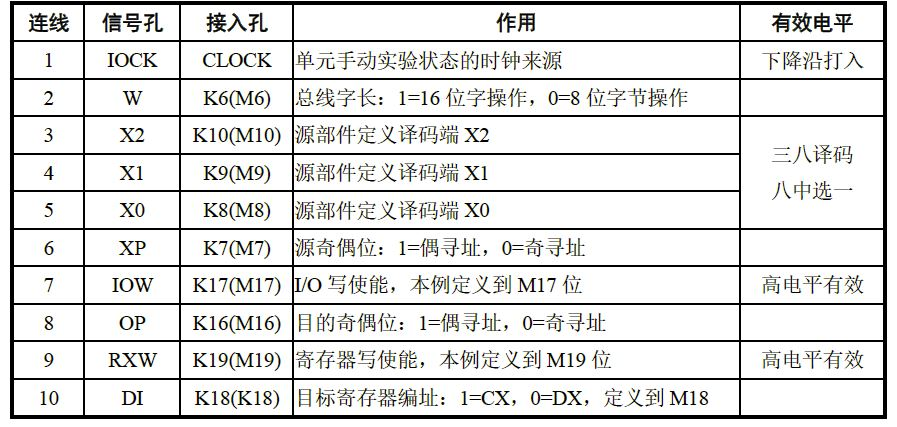
\includegraphics[width=1\textwidth]{lianxian.JPG}
    \caption{寻址定义}
    \label{fig:lianxian}
\end{figure}




搭接的寻址定义如图\ref{fig:dajie}所示,连线方式如图\ref{fig:lianxian}所示。

若 I/O 口为输入端,则 $X_2X_1X_0 = 011$。如何控制奇数偶数位?$W$ 控制字长而 $XP$ 控制是否有偶数位,那么这两个信号孔分别控制奇位和偶位,因此有如下规律 图\ref{fig:jiou}。


\begin{figure}[h]
    \centering
    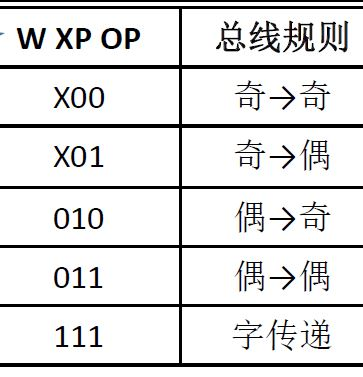
\includegraphics[width=0.5\textwidth]{jiou.JPG}
    \caption{控制奇偶位}
    \label{fig:jiou}
\end{figure}

\section{调试过程、结果与分析}

课程实验要求的数据传输方式如下表\ref{fig:yaoqiu}所示

\begin{figure}[h]
    \centering
    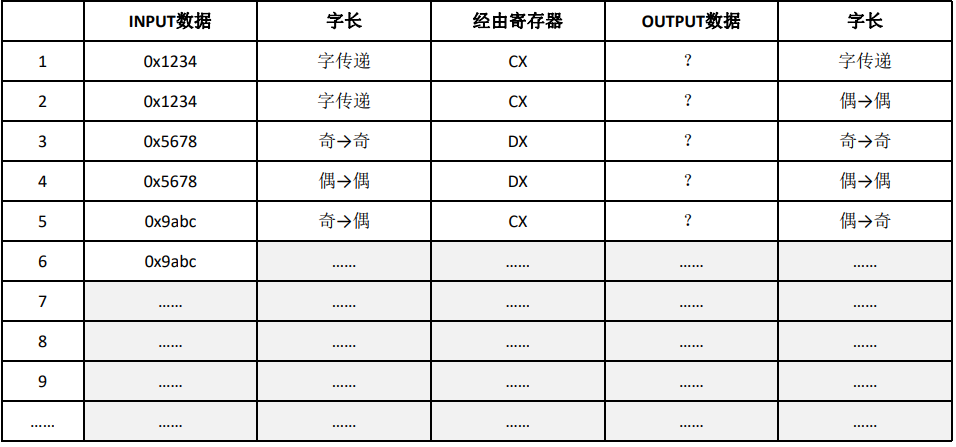
\includegraphics[width=0.8\textwidth]{yaoqiu.PNG}
    \caption{实验要求}
    \label{fig:yaoqiu}
\end{figure}

\subsection{I/O到总线}

无论要求如何,I/O到总线都可分为奇数位到偶数位或者是偶数位到奇数位,或者是仅奇/偶位传输或者是字传输

首先令 $X_2X_1X_0 = 011(IOR)$ 让源部件选择为 I/O,总线会随着 I/O 的变化而变化。根据搭接方式,XP选择 I/O 需要传输的奇偶位,而 OP 选择目的的奇偶位。W 选择传输的总位长。根据图\ref{fig:jiou}我们可以选择自己需要的模式

\subsection{总线到通用寄存器}

通过 DI 选择目的寄存器,DI=1则写CX寄存器,反之写DX寄存器,RXW 寄存器写为 1,然后给 DRCK 一个脉冲。一次脉冲只会有一次随之而来的寄存器写操作。总线到寄存器没有奇偶位的控制选择。

\subsection{寄存器到总线}

通过 SI 选择输入的寄存器,SI=1读入CX寄存器,否则选择DX寄存器,源部件的控制 $X_2X_1X_0 = 110(RRD)$。总线会实时更新为读入寄存器中的值。

\subsection{总线到I/O}

IOW 控制I/O写设为1,然后给 IOCK 一个脉冲,会随着脉冲完成一次总线到I/O的写操作。

\subsection{范例}

实现从I/O偶位的输入到寄存器奇位,再全部输出寄存器到 I/O

\begin{enumerate}
    \item 按[返回]初始化I/O
    \item $X_2X_1X_0 = 011, XP=1,W=0,OP=0$,总线发生变化
    \item $IOW=0, RXW=1, DI=1, OP=1$ 将数据送到 CX,至此输入完成
    \item $X_2X_1X_0 = 110, SI = 1,XP = W = 1$ 总线发生变化,由于这里寄存器只有偶数位,所以字传输还是偶数位传输结果都是一样的
    \item $IOW=1 IOCK$脉冲,I/O口发生变化。此时把所有I/O开关置为1,则能看到输出结果
\end{enumerate}{}

\begin{figure}[h]
    \centering
    \includegraphics[width=0.8\textwidth]{TIM图片20190920120337.jpg}
    \caption{I/O到寄存器CX}
    \label{fig:iocx}
\end{figure}

\begin{figure}[h]
    \centering
    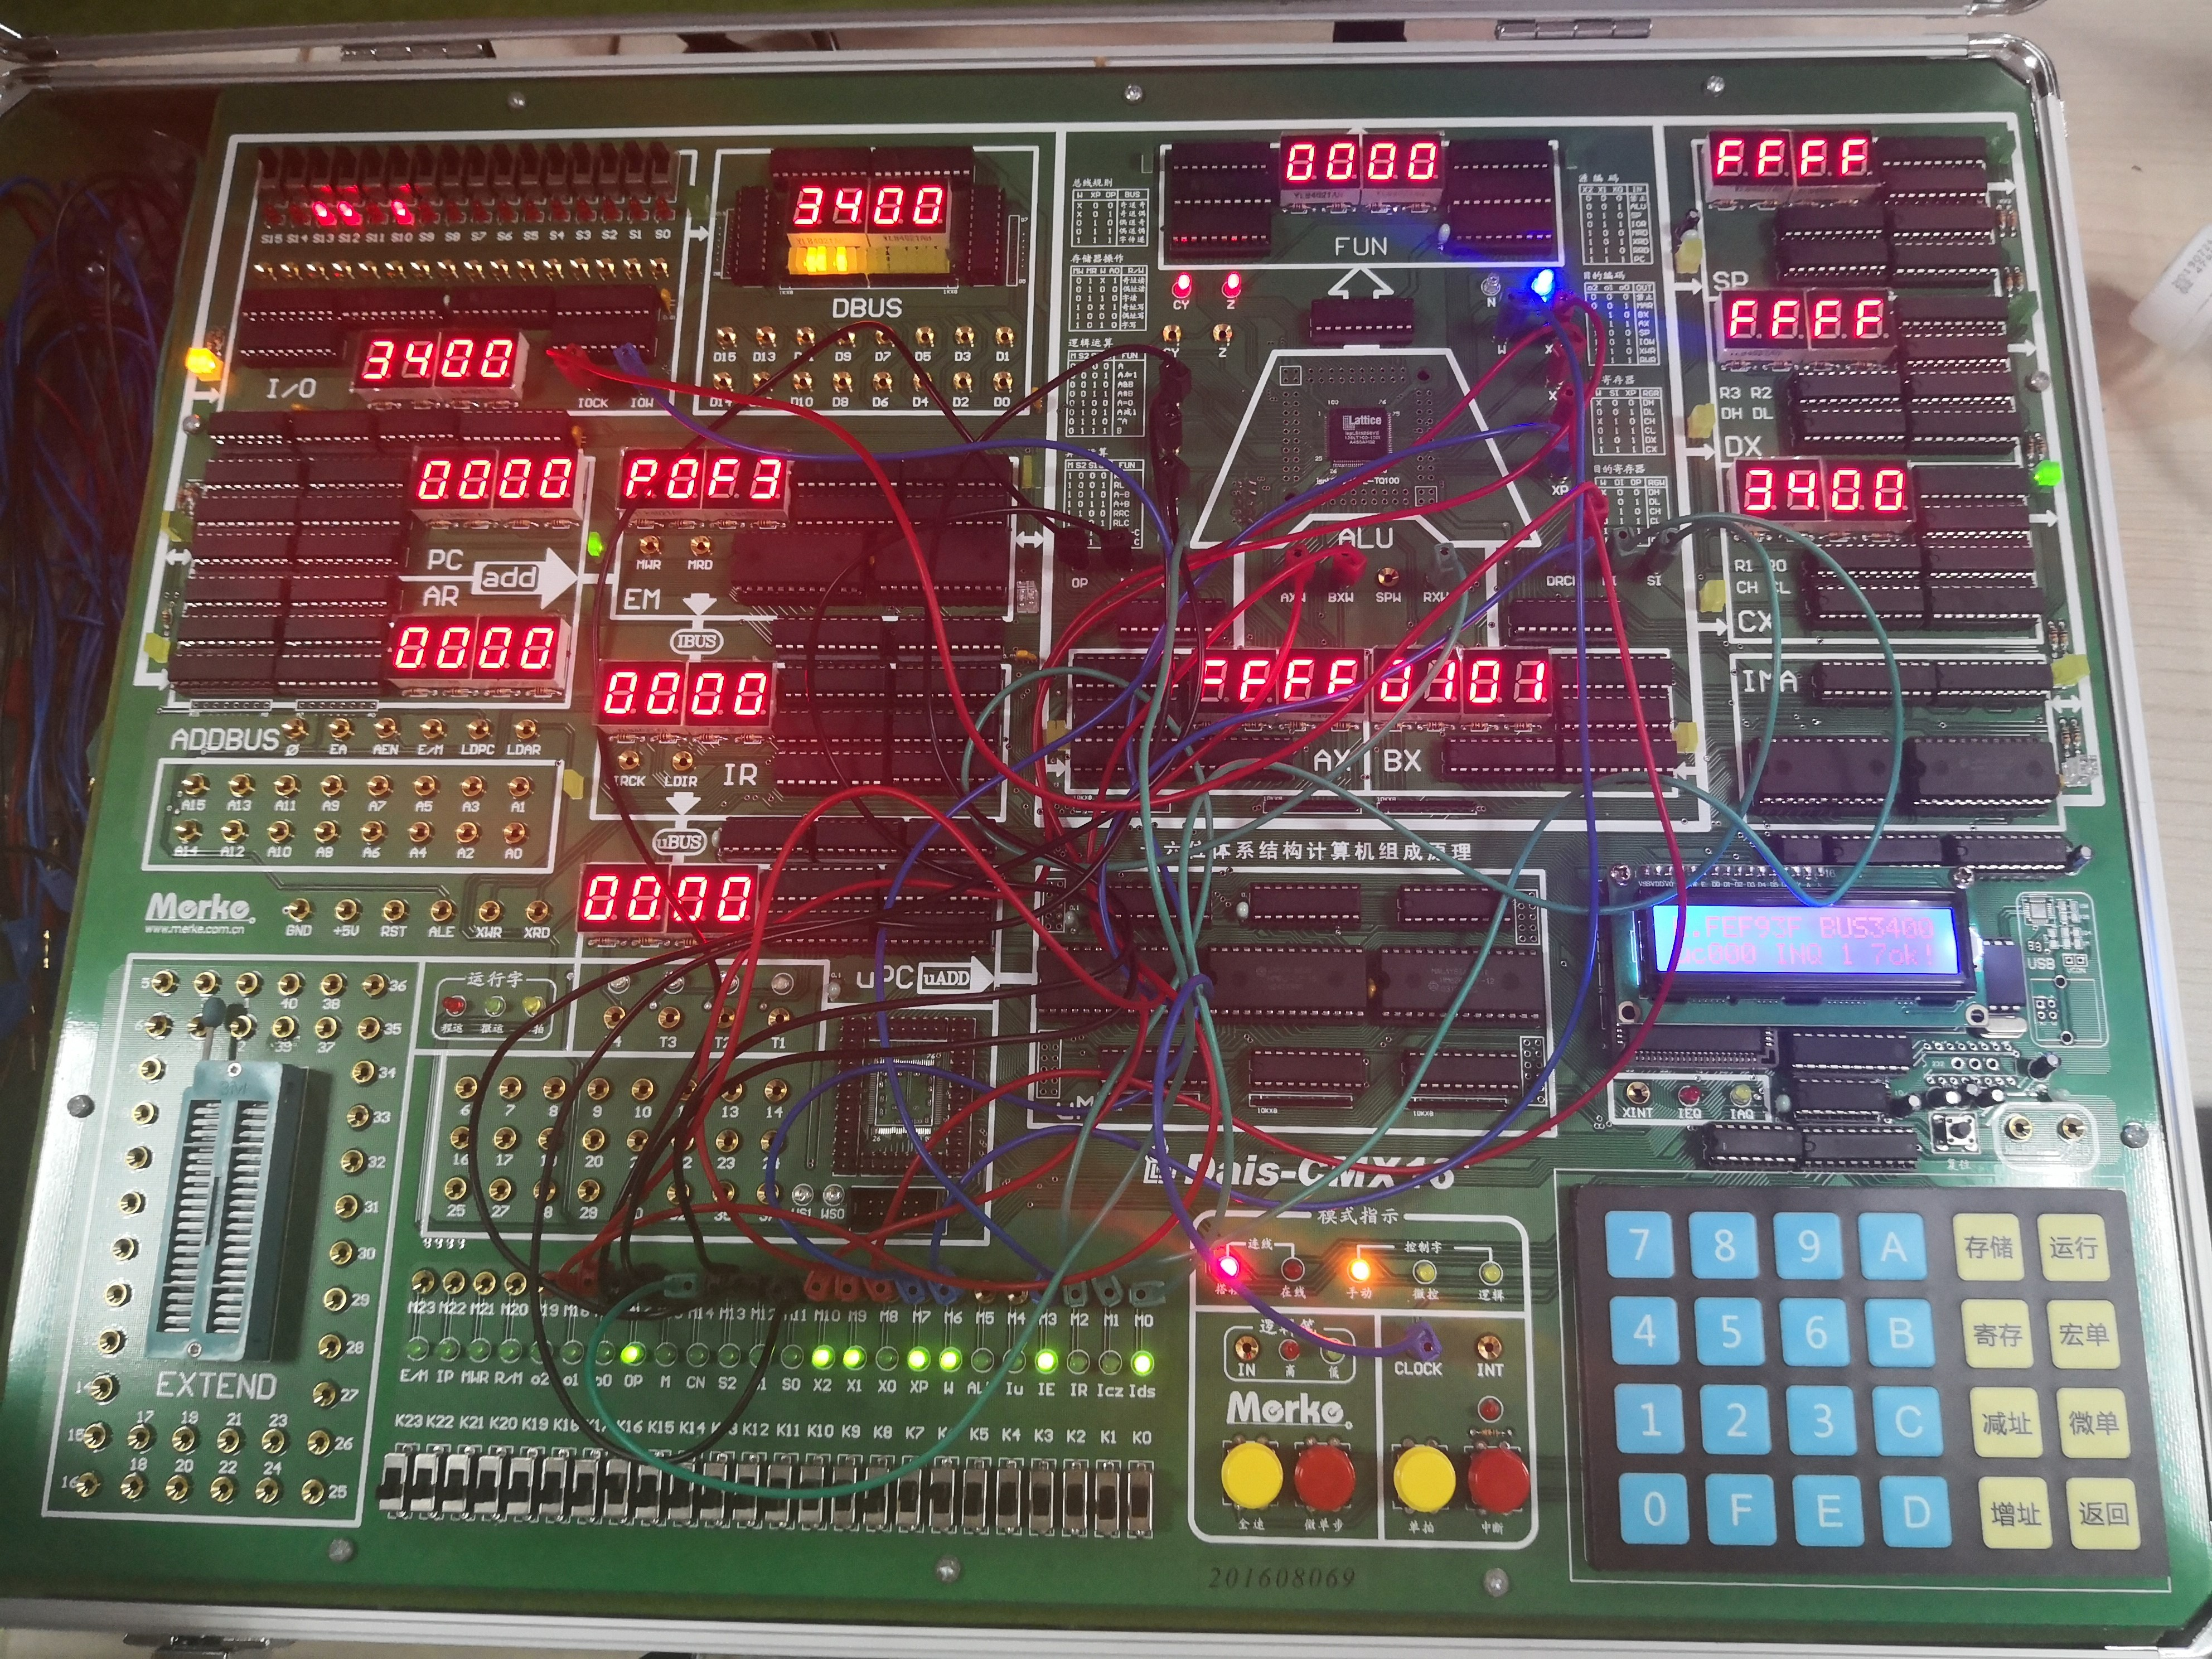
\includegraphics[width=0.8\textwidth]{TIM图片20190920120351.jpg}
    \caption{CX到I/O}
    \label{fig:cxio}
\end{figure}

\subsection{实验结果}

实验结果如图 \ref{tab:outcome} 所示

另外需要说明的是,每次操作我们按返回键进行初始化操作,发现 CX 会初始化为 0000, 而 DX 为 FFFF

\begin{table}[h]
    \centering
    \begin{tabular}{|c|c|c|c|c|c|}
        \hline  & INPUT 数据 & 字长 & 经由寄存器 & OUTPUT 数据 & 字长 \\
        \hline 1 & 0x1234 & 字传递 & CX & 0x1234 & 字传递 \\
        \hline 2 & 0x1234 & 字传递 & CX & 0x0034 & 偶->偶 \\
        \hline 3 & 0x5678 & 奇->奇 & DX & 0x5600 & 奇->奇 \\
        \hline 4 & 0x5678 & 偶->偶 & DX & 0x5600 & 偶->偶 \\
        \hline 5 & 0x9abc & 奇->偶 & CX & 0x9a00 & 偶->奇 \\
        \hline 6 & 0x9abc & 偶->奇 & DX & 0xbc00 & 奇->奇 \\
        \hline 7 & 0x9abc & 奇->偶 & CX & 0x009a & 偶->偶 \\
        \hline 8 & 0x1234 & 字传递 & DX & 0x1200 & 奇->奇 \\
        \hline 9 & 0x1234 & 字传递 & CX & 0x3400 & 偶->奇 \\
        \hline
    \end{tabular}
    \caption{实验结果}
    \label{tab:outcome}
\end{table}{}

\section{总结}

第一次实验总结了以下经验

\begin{enumerate}
    \item 在开始之前最好首先了解每个开关的意义,帮助理解并且减少失误
    \item 开关最好插在下方对应表示的开关口中,剩余的按照表格填入。这样方便记忆每个插口的位置
    \item 每次开始之前先初始化
    \item 仔细阅读实验指导书
    \item 实验箱上每个模块的奇偶位输入都有对应的指示灯,方便指认电路是否连接错误
\end{enumerate}{}

\section{附件}

无
\end{document}
